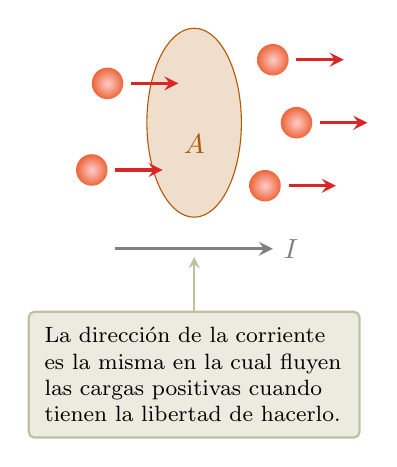
\begin{tikzpicture}[>=stealth]
  \draw[orange!70!black,fill=orange!70!black!20,name=conductor] (0,0) ellipse (0.6 and 1.2) node[below=0.8]{\(A\)};
  \draw[very thick,gray,->] (-1,-1.6) -- (1,-1.6) node[right]{\(I\)};

  \foreach \x\y in {-1.1/0.5,-1.3/-0.6,1/0.8,1.3/0,0.9/-0.8} {
    \shade[inner color=white!80!red, outer color=orange!50!red!70!lightgray] (\x,\y) circle (.2) [radius=1pt];
    \draw[very thick,color=red!70!gray,->] ({\x+0.3},\y) -- ({\x+0.9},\y);
  }

  \node (cartel) [
    font=\footnotesize,
    text width=3.8cm,
    align=left,
    fill=yellow!40!black!14,
    draw=yellow!40!black!46,
    thick,
    rounded corners=2pt,
    inner sep=2mm
    ]
    at (0,-3.2) {La dirección de la corriente es la misma en la cual fluyen las cargas positivas cuando tienen la libertad de hacerlo.};
  \draw[->, thick, color=yellow!40!black!46, shorten >=3pt] 
           (cartel.north) -- (0,-1.6);
\end{tikzpicture}
